\chapter{Introducción}
\label{Introducción}
\section{Introducción}
\\
Los avances tecnológicos y la reducción en los costos en la industria han hecho proliferar la industria aeroespacial, incluyendo la disponibilidad de imágenes satelitales. La lista de proveedores de éstas es extensa e incluye no solo al sector público, cuyas imágenes están disponibles para todos los ciudadanos, sino también, más recientemente, al privado, donde se destacan por ejemplo los sitios Satellogic \cite{satellogic} y Kaggle \cite{kaggle}.
\\

Las imágenes satelitales poseen una serie de particularidades con respecto a otro tipo de imágenes ordinarias (fotografías por ejemplo). Las imágenes satelitales son matrices de varios millones de píxeles, con una basta variedad de resoluciones de terreno, dependiendo del proveedor y de la banda espectral en la que fue obtenida. La resolución de terreno determina el tamaño de los objetos que pueden detectarse en el. Esas imágenes son multiespectrales y existe un arreglo de píxeles por cada banda espectral utilizada. Estos suelen incluir los usuales colores \textit{rojo}, \textit{verde} y \textit{azul} (RGB), pero también \textit{infrarrojos de onda cercana}, \textit{infrarrojos de onda corta}, \textit{termal} o las \textit{bandas pancromáticas} por nombrar algunas. El análisis combinado de estas bandas habilita la construcción y estudio de terreno, tales como vegetación, agua, suelo o termales, que luego facilitan posibles soluciones alrededor de, por ejemplo, el uso del suelo y la detección de suelo cubierto. Las imágenes satelitales son una increíble fuente de información contextual para muchas industrias, sin embargo no es trivial su procesamiento y utilización debido a su alto contenido en información.
\\

Se introduce el concepto de Machine Learning como una disciplina del campo de la Inteligencia Artificial que, a través de algoritmos, dota a los ordenadores de la capacidad de identificar patrones en datos masivos y elaborar predicciones. Deep Learning es una sub-rama de Machine Learning, la cual se basa en usar Redes Neuronales Profundas para encontrar patrones en espacios de grandes dimensiones como son las imágenes satélites. Un modelo de Deep Learning es, a grandes rasgos, un agente flexible que percibe su entorno y lleva a cabo acciones que maximicen sus posibilidades de éxito en algún objetivo o tarea. Dentro de lo que a aplicaciones de Machine Learning se refiere, se destaca la popularidad del uso de Computer Vision  o Visión por computadoras, como uno de los campos de investigación más populares en este momento y se encuentra en la intersección de muchas materias académicas tales como Ciencias de la Computación (Gráficos, Algoritmos, Teoría, Sistemas, Arquitectura), Matemáticas (Recuperación de Información, Aprendizaje Automático, Probabilidad, Estadística), Ingeniería (Robótica, Procesamiento de Imágenes), Física (Óptica), Biología (neurociencia) y Psicología (ciencia cognitiva). 
\\

\subsection{Motivación}
Las tareas de reconocimiento visual como la clasificación, localización y detección de imágenes son utilidades populares que se logran gracias a la aplicación de modelos de Deep Learning. Y es aquí donde el presente proyecto cobra vida: como punto de partida, se conoce que en el territorio argentino, y en particular en las zonas agrícolas se registran diversas infracciones en cuanto a:
\begin{itemize}
    \item Abuso de recursos hídricos.
    \item Evasión impositiva en el rubro agropecuario.
    \item Deforestaciones ilegales.
    \item Asentamientos y expropiaciones ilegales.
\end{itemize}
A su vez, se dispone de un conjunto de imágenes satelitales de público acceso que describen diferentes áreas del territorio argentino. Con ellas se plantea hacer uso de la Ciencia de Datos, el análisis estadístico y Machine Learning para implementar un software que permita analizar el contenido de una imagen satelital y devuelva resultados útiles para la búsqueda de infractores, incorporando de esta forma tecnologías novedosas y altamente populares en la industria al ámbito público. En la actualidad ya se pueden ver usos de tecnologías como la desarrollada en este proyecto, para el uso en el ámbito publico, tal y como se detalla en esta noticia: detección de piscinas no declaradas \cite{noticia} y también explotadas en el ámbito privado como lo hace la siguiente compañía que ofrece diferentes servicios de: Agricultura, Urbanismo y Medio Ambiente \cite{kermap}.

\subsection{Objetivos}
En la siguiente sección se detallan los objetivos a cumplir en el presente proyecto.
\subsubsection{Objetivos Principales}
\begin{itemize}
    \item El objetivo principal del presente trabajo es adquirir conocimientos sobre Deep Learning e Inteligencia Artificial y aplicar dichos conocimientos a desarrollar un prototipo para la detección de imágenes satelitales en un periodo de tiempo corto.\\
    
    \item Ayudar a combatir irregularidades detectándolas fácilmente. En particular detectando pivotes de riego (Figura\ref{fig:pivot}) y silobolsas (Figura \ref{fig:silobolsa}). Ambos utilizados ampliamente en el rubro agrícola.
\end{itemize}

    \begin{figure}
        \centering
        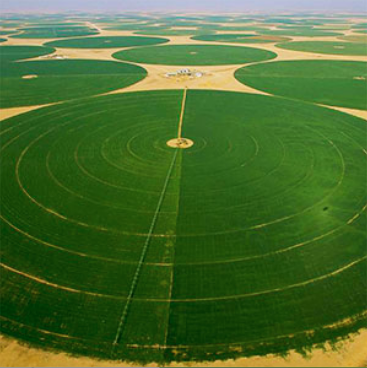
\includegraphics[width=0.7\textwidth]{img/pivot.png}
        \caption{Riegos por pivote (circular): sistema de riego móviles mediante pivotes que permiten regar grandes superficies. Fuente: \cite{img_pivot}}
        \label{fig:pivot}
    \end{figure}
    
    \begin{figure}
        \centering
        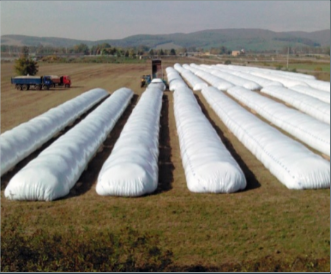
\includegraphics[width=0.7\textwidth]{img/silobolsa.png}
        \caption{Silobolsas: es un sistema que permite almacenar granos secos de maíz, soja, trigo, girasol y arroz en el propio establecimiento productor, a bajo costo y con óptimas condiciones de calidad. Fuente: \cite{img_silo}}
        \label{fig:silobolsa}
    \end{figure}

\subsubsection{Objetivos Particulares}
\begin{itemize}
    \item Investigar sobre Machine Learning y Visión por Computadora, su funcionamiento y sus casos de uso.
    \item Investigar y estudiar diferentes implementaciones de los modelos de Machine Learning más usados en los lenguajes de programación existentes y mejor se apliquen a nuestras necesidades.
    \item Evaluar en base a los requerimientos, cuál es la implementación o framework más adecuado para realizar este prototipo.
    \item Configurar un modelo de Machine Learning en una supercomputadora con los recursos necesarios, en un ambiente de desarrollo e implementarlo en un contenedor Docker \cite{docker} para que sea portable, lo que permite ser instalado en cualquier computadora.
    \item Complementar el prototipo con una API \cite{api} y una interfaz gráfica para mejorar su usabilidad.
\end{itemize}

\subsection{Marco de investigación}
El presente trabajo esta estructurado según el siguiente Workflow:\\
\begin{figure}
    \centering
    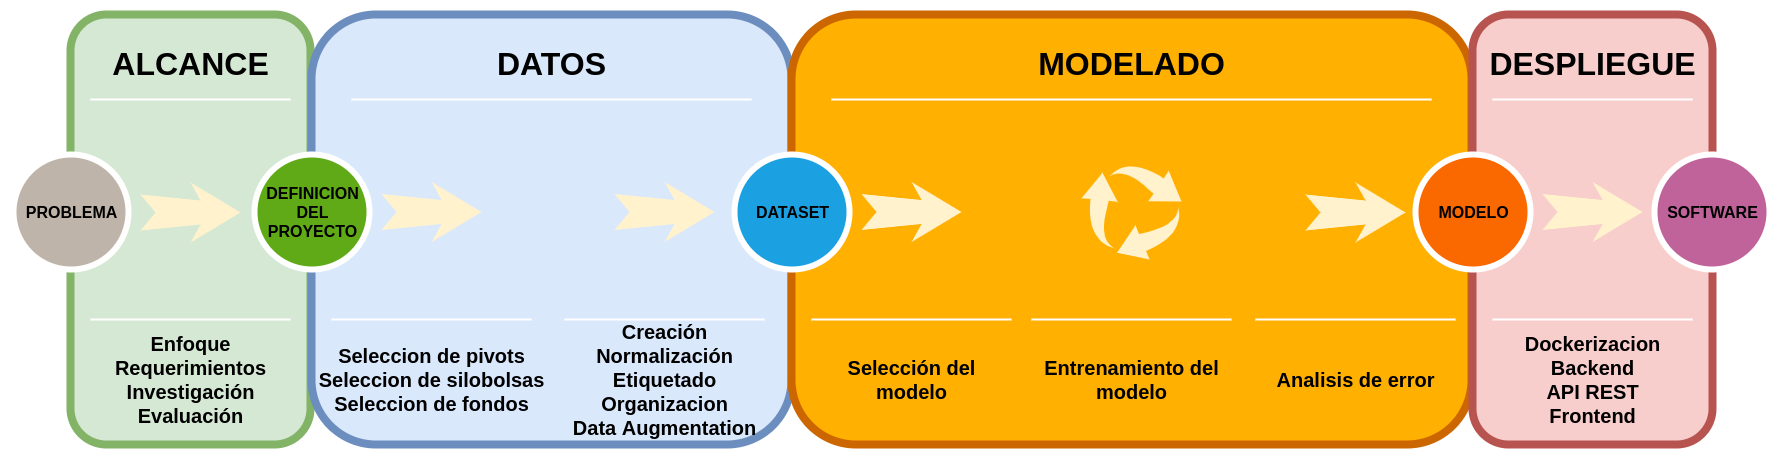
\includegraphics[width=1.2\textwidth,center]{img/Wokflow.drawio.png}
    \caption{Workflow}
    \label{fig:workflow}
\end{figure}

\begin{enumerate}
    \item \textbf{Alcance:} Primero se definió el alcance de nuestro proyecto, para quién estaba enfocado y todo lo necesario para llevarlo a cabo. Se decidió comenzar por una investigación y posterior evaluación de los algoritmos más utilizados para la detección de objetos en tiempo real, con el afán de lograr tiempos de detección reducidos.
    \item \textbf{Datos:} Se continuó con la elección de los datos a utilizar, en este caso imágenes de riegos por pivote y silo bolsas con vista satelital. Se siguió con la creación, normalización y etiquetado de un conjunto de datos, para formar el dataset adecuado.
    \item \textbf{Modelo:} Luego del análisis entre los diferentes modelos más usados, se optó por una primera elección de YOLOv3 (\ref{Estado del Arte - YOLO}), y se procedió con su entrenamiento con los datos previamente seleccionados. Debido a que no se obtuvieron los resultados esperados, se decidió emplear el algoritmo YOLOv5 (\ref{Estado del Arte - YOLO}), que además de tener varias mejoras respecto a la versión 3 resulto ser más efectivo para nuestro problema y se obtuvo un mejor rendimiento.
    
    \item \textbf{Despliegue:} Después se procedió a desarrollar un prototipo de la aplicación con el fin de evaluar la implementación y utilidad de la propuesta. Para eso, el desarrollo se dividió en tres partes:
    \begin{enumerate}
        \item La primera parte consistió en la configuración del Algoritmo YOLOv5 en un entorno virtual contenido en un Docker con los requerimientos y librerías necesarias. Se configuraron 2 entornos virtuales uno para realizar los entrenamientos del algoritmo y dejar corriendo el contenedor Docker con el backend (modelo YOLOv5 + API) y otro entorno con el frontend (página web).
        \item La segunda parte consistió en la programación de la API con la ayuda del framework Flask \cite{flask} para el backend. Se implementaron las siguientes funcionalidades:
        \begin{enumerate}
            \item Subir una imagen nueva o un archivo comprimido con un conjunto de imágenes para ser analizadas.
            \item Consultar la información resultante de cada imagen subida.
            \item Consultar la información y los parámetros del modelo utilizado.
            \item Otorgar la opción de descargar la/s imagen/es analizada/s junto con los resultados de la predicción.
        \end{enumerate}
        \item En la última parte, se desarrolló una aplicación web (Frontend) para que el usuario pueda interactuar con el sistema a través de una interfaz gráfica. Con los siguientes lenguajes de programación: JavaScript, HTML y CSS y el framework Bootstrap \cite{bootstrap}, se le dio estructura y estilo a la página, dando una simple retroalimentación visual al usuario para indicar los resultados de la detección y del análisis.
    \end{enumerate}
\end{enumerate}
\newpage
